\documentclass[11pt]{article}\usepackage[]{graphicx}\usepackage[]{color}
% maxwidth is the original width if it is less than linewidth
% otherwise use linewidth (to make sure the graphics do not exceed the margin)
\makeatletter
\def\maxwidth{ %
  \ifdim\Gin@nat@width>\linewidth
    \linewidth
  \else
    \Gin@nat@width
  \fi
}
\makeatother

\definecolor{fgcolor}{rgb}{0.345, 0.345, 0.345}
\newcommand{\hlnum}[1]{\textcolor[rgb]{0.686,0.059,0.569}{#1}}%
\newcommand{\hlstr}[1]{\textcolor[rgb]{0.192,0.494,0.8}{#1}}%
\newcommand{\hlcom}[1]{\textcolor[rgb]{0.678,0.584,0.686}{\textit{#1}}}%
\newcommand{\hlopt}[1]{\textcolor[rgb]{0,0,0}{#1}}%
\newcommand{\hlstd}[1]{\textcolor[rgb]{0.345,0.345,0.345}{#1}}%
\newcommand{\hlkwa}[1]{\textcolor[rgb]{0.161,0.373,0.58}{\textbf{#1}}}%
\newcommand{\hlkwb}[1]{\textcolor[rgb]{0.69,0.353,0.396}{#1}}%
\newcommand{\hlkwc}[1]{\textcolor[rgb]{0.333,0.667,0.333}{#1}}%
\newcommand{\hlkwd}[1]{\textcolor[rgb]{0.737,0.353,0.396}{\textbf{#1}}}%
\let\hlipl\hlkwb

\usepackage{framed}
\makeatletter
\newenvironment{kframe}{%
 \def\at@end@of@kframe{}%
 \ifinner\ifhmode%
  \def\at@end@of@kframe{\end{minipage}}%
  \begin{minipage}{\columnwidth}%
 \fi\fi%
 \def\FrameCommand##1{\hskip\@totalleftmargin \hskip-\fboxsep
 \colorbox{shadecolor}{##1}\hskip-\fboxsep
     % There is no \\@totalrightmargin, so:
     \hskip-\linewidth \hskip-\@totalleftmargin \hskip\columnwidth}%
 \MakeFramed {\advance\hsize-\width
   \@totalleftmargin\z@ \linewidth\hsize
   \@setminipage}}%
 {\par\unskip\endMakeFramed%
 \at@end@of@kframe}
\makeatother

\definecolor{shadecolor}{rgb}{.97, .97, .97}
\definecolor{messagecolor}{rgb}{0, 0, 0}
\definecolor{warningcolor}{rgb}{1, 0, 1}
\definecolor{errorcolor}{rgb}{1, 0, 0}
\newenvironment{knitrout}{}{} % an empty environment to be redefined in TeX

\usepackage{alltt}

\usepackage[a4paper, margin=2cm]{geometry}

%%%%%%%%%%%%%%%%%%%%%%%%%%%%%%%%%%%%
% %%% for APA6 document class
% \title{QuAX-DaF}
% \shorttitle{Fremdsprachenlehre trifft Quantitative Linguistik}
% \author{Daniel Jach}
% \affiliation{Zhengzhou Universität (Henan, China)}
% \authornote{authornote}
% \abstract{abstract}
% \keywords{keywords}
%%%%%%%%%%%%%%%%%%%%%%%%%%%%%%%%%%%%

%%%%%%%%%%%%%%%%%%%%%%%%%%%%%%%%%%%%
%%% languages
%%%%%%%%%%%%%%%%%%%%%%%%%%%%%%%%%%%%
\usepackage[ngerman]{babel}
\usepackage[utf8]{inputenc}
\usepackage[T1]{fontenc}	 
\usepackage{lmodern} 
\usepackage{CJKutf8} % for Chinese characters
\AtBeginDvi{\input{zhwinfonts}}
\usepackage{pinyin} % for pinyin

%%%%%%%%%%%%%%%%%%%%%%%%%%%%%%%%%%%%
%%% APA 6th
%%%%%%%%%%%%%%%%%%%%%%%%%%%%%%%%%%%%
\usepackage[style=apa, backend=biber,natbib]{biblatex} 
\usepackage{csquotes}
\DeclareLanguageMapping{american}{american-apa}

\usepackage{sectsty} % style headings
\subsubsectionfont{\normalfont\itshape} % italicize level 4 subsubsection headings 

%%%%%%%%%%%%%%%%%%%%%%%%%%%%%%%%%%%%
%%% plots
%%%%%%%%%%%%%%%%%%%%%%%%%%%%%%%%%%%%
\usepackage{tikz} 
\usetikzlibrary{decorations.fractals}
\usepackage{tikz-qtree} % for trees
\usepackage{import}

\usepackage{caption} 
\usepackage[labelformat=simple]{subcaption} % for subfigures side by side
\captionsetup{labelfont=bf,textfont=normalfont,singlelinecheck=off,justification=raggedright}

\usepackage{graphicx}
\usepackage{xcolor,colortbl}
%%%%%%%%%%%%%%%%%%%%%%%%%%%%%%%%%%%%
%%% linguistic examples, glosses
%%%%%%%%%%%%%%%%%%%%%%%%%%%%%%%%%%%%
\usepackage{expex} 
\gathertags % for forward reference with expex


%%%%%%%%%%%%%%%%%%%%%%%%%%%%%%%%%%%%
%%% bibliography
%%%%%%%%%%%%%%%%%%%%%%%%%%%%%%%%%%%%
\bibliography{./quax-daf.bib} % bibliography source

%%%%%%%%%%%%%%%%%%%%%%%%%%%%%%%%%%%%
%%% tables 
%%%%%%%%%%%%%%%%%%%%%%%%%%%%%%%%%%%%
\usepackage{booktabs} % for better tables
\usepackage{multirow} % for multirow cells in tables
\usepackage{tabu} % for textwidth tables with kable
\usepackage{threeparttablex} % for tablenotes in tabu tables
\usepackage{threeparttable} % for tablenotes in normal tabular tables
\usepackage{tabularx} % for pagewidth tables
\usepackage{rotating} % for sidewaystables
%%%%%%%%%%%%%%%%%%%%%%%%%%%%%%%%%%%%
%%% rest 
%%%%%%%%%%%%%%%%%%%%%%%%%%%%%%%%%%%%
\usepackage{setspace} 
\onehalfspacing
\usepackage{mathtools} % for mathematical symbols
\usepackage{nicefrac} % for nice fractions
\setcounter{secnumdepth}{5} % level of numbering
\usepackage{amssymb} % for certain symbols, e.g., $\varnothing$
\usepackage[multiple]{footmisc} % for two or more footnotes at one point
\usepackage{wrapfig} % for wrapping figures in text
\usepackage{amsmath} % for boxes and all kinds of math things
\usepackage{amssymb}
\usepackage{amsfonts}
\usepackage{footmisc} % for repeating footnotes
\usepackage{lipsum} % for dummy text
\usepackage{pdfpages} % for including pdf pages
\usepackage[hidelinks]{hyperref} % for hyperlinks
\hypersetup{
    colorlinks,
    linkcolor={red!50!black},
    citecolor={blue!50!black},
    urlcolor={blue!80!black}
}


\usepackage{titlesec} % for styling section headings

\titleformat{\section}
  {\fontfamily{phv}\bfseries}{\thesection}{1em}{}
\titleformat{\subsection}
  {\normalfont\bfseries}{\thesubsection}{1em}{}
\titleformat{\subsubsection}
  {\normalfont}{\thesubsubsection}{1em}{}


\setcounter{biburlnumpenalty}{100}  % allow breaks at numbers
\setcounter{biburlucpenalty}{100}   % allow breaks at uppercase letters
\setcounter{biburllcpenalty}{100}   % allow breaks at lowercase letters


% abbreviations:
\usepackage[acronym]{glossaries}
\newacronym{2WYP}{2WYP}{two-way prepositions}


\usepackage{lastpage}
\usepackage{fancyhdr}
\pagestyle{fancy} 
\fancyhf{}
\chead{QuAX-DaF -- Quantitative Analyse von Texten für den DaF-Unterricht -- Daniel Jach}
\rhead{}
\lhead{}
\cfoot{Seite \thepage~von~\pageref*{LastPage}}
\lfoot{}


\hyphenation{ent-hält deutsch-sprachige Niveau-stufen ein-ge-stell-ten}

% \usepackage{draftwatermark}
% \SetWatermarkText{Manuskript}
% \SetWatermarkScale{1}
\IfFileExists{upquote.sty}{\usepackage{upquote}}{}
\begin{document}
\captionsetup[figure]{name={Abb.}}










\thispagestyle{empty}


  \begin{titlepage}
    \vspace*{\fill}
    \begin{center}
      {\Huge QuAX-DaF}\\[0.5cm]
      {\Large Quantitative Analyse von Texten\\für den Deutsch-als-Fremdsprache-Unterricht}\\[2cm]
      {\Large Daniel Jach}\\[2cm]
      Letzte Änderung\\10. Oktober 2020\\[2cm]
    \end{center}
    \vspace*{\fill}
  \end{titlepage}






\newpage

\section{Einleitung}

QuAX-DaF (\textbf{Qu}antitative \textbf{A}nalyse von Te\textbf{X}ten für \textbf{D}eutsch \textbf{a}ls \textbf{F}remdsprache) ist ein online Werkzeug für den DaF-Unterricht, erreichbar unter \href{https://danieljach.shinyapps.io/quax-daf/}{https://danieljach.shinyapps.io/quax-daf/}. Das Programm analysiert deutschsprachige Texte mit Methoden der quantitativen Linguistik und erzeugt Material für Übungen zum Textverstehen und Wortschatzerwerb, angepasst an den Vokabelstand Ihrer Lernenden. QuAX ist für Lehrerinnen und Lehrer gemacht, möglichst praktikabel gestaltet und verlangt kein linguistisches oder statistisches Vorwissen. QuAX ist meines Wissens das erste DaF-Tool, das auf Erkenntnissen der gebrauchsbasierten Spracherwerbsforschung aufbaut und diese für den Unterricht nutzbar macht. 

\section{Gebrauchsbasierter Spracherwerb, Textverstehen und Wortschatz}

Ergebnisse psycholinguistischer Forschung haben gezeigt, dass eine Fremdsprache -- ähnlich wie eine Muttersprache -- zu wesentlichen Teilen aus dem Gebrauch heraus gelernt wird \parencites{Ellis.2015,Madlener.2015}. Solches erfahrungsbasiertes Lernen ist ein Nebenprodukt mentaler Aktivität und verläuft normalerweise implizit, das heißt ohne dass die Lernenden etwas davon mitbekommen. Gebrauchsbasierte Forschung geht dabei davon aus, dass Lernende einzelne Äußerungen, die ihnen im Sprachgebrauch begegnen, im Gedächtnis behalten und unbewusst hinsichtlich Form und Bedeutung miteinander vergleichen. Wiederkehrende Gemeinsamkeiten schreiben sich tiefer ins Gedächtnis ein, so dass sich sukzessive schematische Abbilder (Repräsentationen) geteilter grammatischer und anderer Eigenschaften herausbilden. Diese gebrauchsbasierten Abbilder unterscheiden sich von ihren Lehrbuch-Beschreibung wie Wildtiere von ihren im Zoo lebenden Artgenossen: Sie sind auf ihre Umgebung feinabgestimmt und in ein enges Netz ähnlicher Konstruktionen eingebunden \parencites{Diessel.2019,Roemer.2004,Wagner.2015}. Die Häufigkeit, mit der eine bestimmte Konstruktion im Input erscheint, ist dabei ein entscheidender Faktor für ihren Erwerb und die Ausgestaltung ihrer Repräsentation \parencites{Diessel.2016,Schmid.2018}. 

Der gebrauchsbasierte Ansatz ist nicht auf den Erwerb grammatischer Konstruktionen beschränkt, sondern bezieht auch den Erwerb von Wörtern ein. Korpuslinguistische Arbeiten haben etwa gezeigt, dass Wörter in Texten nicht wie einzelne Bausteine aneinander gereiht, sondern normalerweise in einem mehr oder weniger engen Verbund mit anderen Wörtern gebraucht werden \parencites{Hoey.2004,Sinclair.1991}. Erwerb und Verarbeitung solcher Kollokationen hängen wiederum wesentlich von der Häufigkeit ab, mit der Lernende ihnen begegnen \parencite{Schmitt.2012}. Auch konnotative Anteile der Wortbedeutung werden überwiegend beiläufig aus dem Gebrauch heraus gelernt \parencite{Corrigan.2004}. 

Auf diese Weise erwerben Lernende die Wörter und grammatischen Konstruktionen einer Sprache implizit aus ihren Gebrauchserfahrungen, ähnlich einem neuronalen Netzwerk, das wiederkehrende Muster in seinem Input erkennt, intern abspeichert und die entstehenden Abbilder kontinuierlich nachbessert, ohne dafür eines ``Bewusstseins'' zu bedürfen oder ein solches zu entwickeln \parencite{Elman.1993}. Damit werden die Existenz bewusster Lernvorgänge und die Wichtigkeit von Instruktionen keineswegs verneint, sondern ihre Rolle wird im Zusammenspiel mit impliziten Prozessen bestimmbar. Instruktionen haben in diesem Modell vor allem die Funktion, den Lernenden auf noch unbekannte Strukturen in seinem Input aufmerksam zu machen. Bewusste Lernvorgänge steuern ihre Verarbeitung so lange, bis sich ein internes Abbild herausbildet, das diese Aufgabe automatisch und unbewusst übernimmt \parencites{Ellis.2015b,Roehr-Brackin.2018}.

Für den Erwerb realistischer Konstruktionen und ihre idiomatische Feinabstimmung auf den Kontext ist also Erfahrung mit authentischem Sprachgebrauch von besonderer Bedeutung. Im gesteuerten Fremdsprachenerwerb im Herkunftsland ist authentischer Sprachgebrauch vor allem in Form von Texten (und aufgezeichneten Gesprächen) für Lernende erfahrbar. In bildungssprachlichen Domänen, zum Beispiel in der universitären Erwachsenenbildung, in der Vorbereitung auf ein Studium im Ausland oder im deutschsprachigen Fachunterricht an Auslandsschulen, dominieren Texte mit bildungs-, fach- und schriftsprachlichen Registern. Das Verstehen solcher Texte setzt aber normalerweise schon einen relativ großen Wortschatz voraus \parencite{Tschirner.2019}. Relevant für das Textverstehen sind zum einen besonders häufige Wörter, weil diese mehr als seltene Wörter zur Textdeckung beitragen \parencite{Nation.2006}. Korpuslinguistische Studien haben jedoch gezeigt, dass die oft für den Unterricht herangezogenen pragmatisch orientierten Wortlisten (zum Beispiel Langenscheidt, Goethe-Institut, Profile Deutsch) nur einen kleinen Teil solcher Wörter enthalten. Genauer gesagt: Statt häufiger Wörter, die wesentlich zum Textverstehen beitragen, enthalten diese Listen überwiegend relativ seltene Wörter, die meist für direkte Gespräche in bestimmten Alltagsdomänen gedacht sind \parencite{Tschirner.2006}. Auch ein häufigkeitsbasierter DaF-Vokabeltrainer existiert bislang nicht. Zum anderen spielen Wörter bildungs-, fach- und schriftsprachlicher Register eine entscheidende Rolle. Solche Wörter sind in den einschlägigen Wortlisten gewöhnlich nicht enthalten und kommen auch nur selten in alltagssprachlichen Texten vor. Sie sollten im Unterricht daher hervorgehoben und ihr Gebrauch gezielt vermittelt werden. 

\section{QuAX-DaF}

\subsection{Funktionsweise}

QuAX nutzt Methoden und Einsichten der gebrauchsbasierten Spracherwerbsforschung, um deutschsprachige Texte statistisch zu analysieren und für den DaF-Unterricht auf unterschiedlichen Niveaustufen aufzubereiten. Eingegebene Texte werden zunächst lemmatisiert, das heißt flektierte Wortformen werden in ihre Grundform (Lemma) gebracht. Anschließend vergleicht QuAX die Häufigkeit der Wörter im Text mit ihrer Häufigkeit im Deutschen und bildet den Vergleich anschaulich ab. Das ermöglicht es den Lehrenden einzuschätzen, ob der eingegebene Text vor allem gebräuchliche oder ungewöhnlich viele seltene Wörter enthält und welche das sind. 

Angepasst an den Vokabelstand der Lernenden erzeugt QuAX dann automatisch Übungsmaterial für den typischen unterrichtspraktischen Dreischritt: vor dem Lesen, beim Lesen und nach dem Lesen \parencite[20]{Watkins.2017}. 

\subsection{Textanalyse}

QuAX eignet sich zur Analyse ganz unterschiedlicher bildungssprachlicher Texte, zum Beispiel sprach- und literaturwissenschaftlicher Fachtexte, journalistischer Nachrichten, Rezensionen und Reportagen, literarischer Werke oder Texte für den deutschsprachigen Fachunterricht. Geben Sie im Steuerungspaneel (siehe Abbildung~\ref{figure:QuAX_side}) einen Text in das dafür vorgesehene Feld ein oder laden Sie einen Text im PDF-Format hoch. Sie können auch einen vorbereiteten Beispieltext aus der Dropdown-Liste darunter auswählen. Die Beispiele enthalten Texte, wie sie etwa in deutschsprachigem Geschichtsunterricht, Übungen zum Textverstehen oder sprach- und literaturwissenschaftlichen Seminaren im universitären DaF-Unterricht zum Einsatz kommen. Eine Analyse ist aus statistischen Gründen nur möglich, wenn Ihr Text eine gewisse Länge und Komplexität aufweist. 

Wählen Sie für dieses Beispiel den Text \textit{Kinderzeitmaschine: Über Ritter} aus. Der Text ist eine Zusammenstellung mehrerer Beiträge zum Thema \textit{Ritter}, die auf der öffentlich geförderten Webseite \textit{\url{https://www.kinderzeitmaschine.de/}} erschienen sind und sich an Kinder im Alter zwischen acht und dreizehn Jahren wenden. Der Text erscheint im Eingabefeld. Klicken Sie anschließend auf die Schaltfläche \textit{Analyse beginnen} und zählen Sie leise bis zehn.

\begin{wrapfigure}{L}{0.5\textwidth}
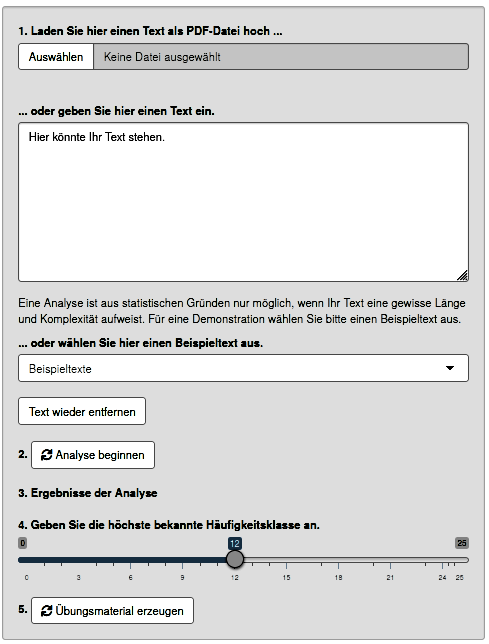
\includegraphics[width=0.5\textwidth]{QuAX_side.png}
\caption{Steuerungspaneel}
\label{figure:QuAX_side}
\end{wrapfigure}

QuAX lemmatisiert die Textwörter, ermittelt ihre Häufigkeit im Text und vergleicht sie mit ihrer Häufigkeit im Deutschen. Das Ergebnis der Analyse erscheint rechts neben dem Steuerungspaneel (siehe Abbildung~\ref{figure:QuAX_results}). 

Das Programm ermittelt die Anzahl der einzelnen Wörter in Ihrem Text (Tokens) und vergleicht sie mit der Anzahl verschiedener Wörter (Types). Das Type-Token-Verhältnis ist ein in der Korpuslinguistik häufig genutztes Maß, um die Komplexität eines Textes einzuschätzen. Der Wert steigt mit der Anzahl der Types und fällt mit der Anzahl der Tokens. Der analysierte Text erreicht einen Wert von 0,5. Das bedeutet, dass durchschnittlich jeder Type zweimal im Text als Token vorkommt. Zum Vergleich wird das Type-Token-Verhältnis in den "`Sternchen"'-Texten der bekannten PASCH-Initiative angezeigt\footnote{\url{https://www.pasch-net.de/de/pas/cls/leh/unt/dst.html}, heruntergeladen am 2. Januar 2020.}, geordnet nach den Niveaustufen des Gemeinsamen Europäischen Referenzrahmens (GER). Der analysierte Text liegt zwischen den Niveaustufen B2/C1 und C1. Probieren Sie einige andere Beispieltexte aus. Der zweite Beispieltext, das Grimmsche Märchen \textit{Rumpelstilzchen}, zum Beispiel liegt mit einem Type-Token-Verhältnis von 0,4 auf einem Niveau mit den PASCH-Texten der Niveaustufe B1. Die Reportage \textit{Zu Hause im Baumhaus} übersteigt mit einem Wert von 0,57 den Wert der C1-PASCH-Texte. Relativ hohe Werte können auch von der Kürze der analysierten Texte bedingt sein. Ein längerer Auszug aus Siegfried Lenz' Roman \textit{Deutschstunde} etwa, ein ohne Zweifel für fremdsprachige Leser schwieriger Text, erzielt mit 0,41 einen relativ niedrigen Wert, weil sich Types in längeren Texten häufiger wiederholen. 

Anschließend werden Textwörter angezeigt, die QuAX unbekannt sind. Hier erscheinen häufig Eigennamen, technische Ausdrücke, Fremdwörter und seltene Nomen-Komposita. Im \textit{Ritter}-Text sind QuAX zum Beispiel die Wörter \textit{Lehnsherren, Schwertgürtel, Schwertleite, Kampfübungen, Nasalhelm} und \textit{Kettenhaube} unbekannt. Außerdem werden im Gegenwartsdeutsch nicht mehr gebräuchliche Wörter wie \textit{Turnei} und \textit{Tjost} und äußerst seltene Wörter wie die Präteritum-Plural-Form \textit{schützten} angezeigt. Daneben kommt es hin und wieder zu Missverständnissen. Zum Beispiel erkennt QuAX nicht, dass \textit{Das} und \textit{Die} Artikelwörter am Satzanfang bzw. am Beginn einer Überschrift sind. Bei der Analyse von Fachtexten werden hier auch Fachausdrücke aufgelistet. Aus der Definition von \textit{Hermeneutischer Zirkel} etwa sind QuAX unter anderem die Wörter \textit{Zirkelbewegung, Textverstehen, wirkungsgeschichtliches} und \textit{Verstehenskonstituenten} nicht bekannt. 

Wie sollten Sie mit diesen Wörtern im Unterricht umgehen? Das hängt auch von Ihren Lernzielen ab. Einige Wörter könnten im Text durch andere Ausdrücke ersetzt werden (z.B. \textit{Kettenhaube} und \textit{Nasalhelm} durch \textit{Schutzhaube} und \textit{Helm}), um die Lektüre zu vereinfachen. Andere Wörter beziehen sich auf sachlich relevante Konzepte, die vor der Lektüre eingeführt werden sollten (z.B. \textit{Lehnsherr}). Wieder andere Wörter sachlich relevanter Konzepte sollten die Lernenden durch die Lektüre selbstständig erschließen (z.B. \textit{Turnei} und \textit{Tjost}, die im Text erklärt werden). Und Fachvokabular (z.B. \textit{Textverstehen} und \textit{Verstehenskonstituenten} aus dem \textit{Hermeneutik}-Textbeispiel) könnten die Lernenden selbstständig während der Lektüre in Fachwörterbüchern nachschlagen. 

Das anschließende Diagramm vergleicht den eingegebenen Text mit dem Deutschen. Die Punkte stehen für die Lemmas im Text. Die Lemmas erscheinen, wenn Sie mit der Maus über die Punkte fahren. Ihre Häufigkeit im Text ist auf der horizontalen Achse abgetragen, ihre Häufigkeit im Deutschen auf der vertikalen Achse. Das Wort \textit{Ritter} zum Beispiel ist im analysierten Text häufig, im Deutschen dagegen eher selten, und erscheint dementsprechend in der rechten unteren Ecke des Diagramms. Angezeigt wird nicht die absolute Häufigkeit, sondern (grob gesagt) wie häufig oder selten ein Wort im Text bzw. im Deutschen verglichen mit einem durchschnittlich häufigen Wort vorkommt. Sogenannte Stoppwörter, die für den Textinhalt eine untergeordnete Rolle spielen, zum Beispiel \textit{aber, am, denn, diesen, keine, manche, sonst, unser} und \textit{zwischen}, wurden aussortiert, weil sie besonders häufig auftreten und das Diagramm darum stark verzerren würden. Sie können das Diagramm bewegen und heranzoomen (Werkzeugleiste).

\begin{figure}
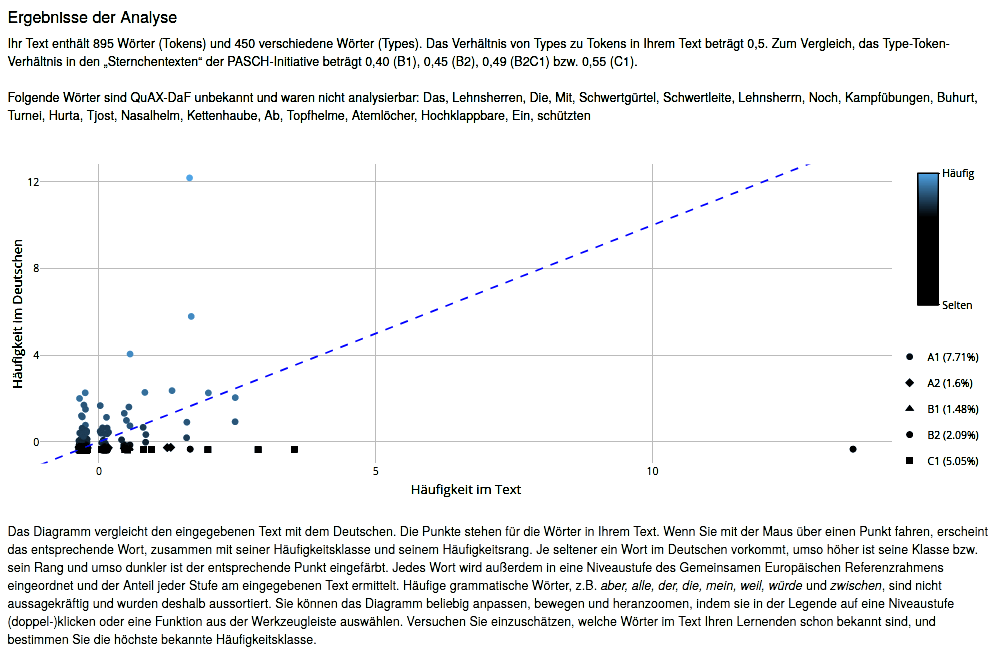
\includegraphics[width=\textwidth]{QuAX_results.png}
\caption{Ergebnisse der Analyse}
\label{figure:QuAX_results}
\end{figure}

Wörter, die im Deutschen häufig, aber im Text relativ selten vorkommen, erscheinen oberhalb der blauen Linie. Hierzu gehören im Beispieltext etwa \textit{geben, sollen, kommen, neu, sagen, Jahr} und die Verschmelzungen von \textit{in} und \textit{zu} mit Artikelwörtern zu den Formen \textit{im} und \textit{zum}. Diese Wörter verursachen vermutlich keine besonderen Verstehensschwierigkeiten. Sofern sie Ihren Lernenden aber noch nicht bekannt sind, sollten diese Wörter vorrangig gelernt werden. Sie sind zwar im untersuchten Text relativ selten, kommen aber in anderen Texten umso häufiger vor und tragen dort wesentlich zur Textdeckung bei.

Wörter, die im Deutschen selten, aber im Text relativ häufig vorkommen, erscheinen unterhalb der blauen Linie. Sie verdienen besondere Aufmerksamkeit. Sie tragen zur Textdeckung bei und spielen inhaltlich vermutlich eine wichtige Rolle in Ihrem Text. Dazu gehören im \textit{Ritter}-Text die Wörter \textit{Ritter, Schwert, Lanze, Knappe, Schild} und \textit{Jahrhundert}. Eine Analyse von Grimms Märchen \textit{Rumpelstilzchen} platziert an dieser Position bezeichnenderweise die Wörter \textit{Männchen, Stroh, Gold} und \textit{spinnen}. Die häufige direkte Rede im Märchentext zeigt sich in der überproportionalen Verwendung von \textit{sprechen} (z.B. \textit{Der König sprach zum Müller: ...}). Ein Auszug aus Anne Franks Tagebuch enthält besonders häufig die Wörter \textit{Vater, Mutter} und den Namen von Annes Schwester, \textit{Margot}, aber auch \textit{Haus}, \textit{kommen} und \textit{gehen} kommen relativ häufig vor. Bei der Analyse von Fachtexten wie der Definition von \textit{Hermeneutischer Zirkel} erscheint hier unter anderem fachspezifische Terminologie, die im normalen Sprachgebrauch nur selten verwendet wird, zum Beispiel \textit{Text, Zirkel, Interpretation} und \textit{Spirale}. Diese Wörter sind im Deutschen selten, erscheinen im untersuchten Text aber überproportional häufig und scheinen besonders prägend für den untersuchten Text zu sein. 

Am Achsenschnittpunkt sammeln sich Wörter, die sowohl im Deutschen als auch im Text relativ selten sind, in einer dichten Wolke. Hierzu gehören im \textit{Ritter}-Text zum Beispiel \textit{kämpfen, lernen, Gesicht, allein, Holz, Gedicht, Krieg, dreieckig, zusammenbauen} und \textit{ernennen}. Je größer und dichter diese Wolke ist, umso mehr verschiedene Wörter enthält der Text, einen umso größeren Wortschatz verlangt er von den Lernenden und umso schwieriger ist er dementsprechend zu verstehen. 

Zusammen mit den Lemmas werden ihre Häufigkeitsklasse, ihr Häufigkeitsrang und eine Einordnung in die Niveaustufen des GER angezeigt. Je seltener ein Wort im Deutschen vorkommt, umso höher ist seine Häufigkeitsklasse und umso heller ist der entsprechende Punkt eingefärbt. Der Häufigkeitsrang bildet einen ähnlichen Zusammenhang kleinschrittiger ab, ist aber nicht so robust wie die Häufigkeitsklasse. Das Wort \textit{Ritter} zum Beispiel erreicht die Häufigkeitsklasse 13 und den Häufigkeitsrang 3.248, beides relativ hohe Werte, die anzeigen, dass \textit{Ritter} im Gebrauchsdeutsch der Gegenwart eher selten vorkommt. 

Die GER-Niveaustufen werden mit verschiedenen Formen angezeigt, die in der Legende neben dem Diagramm beschrieben sind. Das Wort \textit{Ritter} etwa wird der Niveaustufe C1 zugeordnet und erscheint im Diagramm daher als Quadrat. Wenn Sie in der Legende auf eine bestimmte Niveaustufe klicken, werden Wörter dieser Stufe aus dem Diagramm entfernt. Wenn Sie einen Doppelklick ausführen, werden nur Wörter dieser Stufe angezeigt. In der Legende wird auch der Anteil der Wörter verschiedener Niveaustufen im eingegeben Text angezeigt. Im \textit{Ritter}-Text werden 15,59\% der Textwörter auf dem Niveau C1 eingeordnet, 6,45\% dem Niveau B2, 4,57\% dem Niveau B1, usw. Diese Einordnung basiert \textit{nicht} auf den pragmatisch orientierten Wortlisten des Goethe-Instituts, sondern auf dem Häufigkeitsrang der Wörter. Nach einer korpuslinguistisch gestützten Einschätzung von \citet[101]{Tschirner.2019} wächst der Wortschatz von Lernenden mit ihrem GER-Niveau ungefähr wie in Tabelle~\ref{table:GER} abgebildet. 


\begin{table}[htbp]
\centering
\begin{threeparttable}
\caption{Zusammenhang von GER-Niveau und Wortschatz-Größe}
\label{table:GER}
\begin{tabular}{lccccc}
\toprule
GER-Niveau & A1 & A2 & B1 & B2 & C1 \\
\midrule
Wortschatz & 800 & 1600 & 3200 & 4000 & 5500 \\
\bottomrule
\end{tabular}
\end{threeparttable}
\end{table}

\noindent QuAX ordnet dementsprechend die 800 häufigsten deutschen Wörter auf Niveau A1 ein, Wörter mit einem Häufigkeitsrang zwischen 801 und 1600 auf Niveau A2, usw. Ab einem Häufigkeitsrang von 4001 hat ein Wort das Niveau C1 erreicht. 

Bestimmen Sie jetzt den Vokabelstand Ihrer Lernenden. Versuchen Sie einzuschätzen, welche Wörter im Text Ihren Lernenden schon bekannt und welche ihnen noch unbekannt sind, und ermitteln Sie so die höchste bekannte Häufigkeitsklasse. Wenn Ihren Lernenden zum Beispiel die Wörter \textit{Ritter, Schild, Schwert, Gebrauch, Nase} und \textit{Mut} schon bekannt sind, dann haben sie wahrscheinlich auch andere Wörter derselben Klasse (13), zum Beispiel \textit{Wettkampf, Metall, Gesang, Ehre} und \textit{erfreuen} sowie häufigere Wörter niedrigerer Klassen, etwa \textit{Holz, Pferd, tödlich, Schlag} und \textit{klein}, schon größtenteils erworben. Textwörter höherer Klassen (zum Beispiel \textit{Langschwert, Lehnsherr, durchbohren, maßvoll, Lanze, adlig} und \textit{Lösegeld}) sind ihnen dagegen möglicherweise nur vereinzelt oder nicht bekannt. Die höchste Ihren Lernenden noch bekannte Häufigkeitsklasse, zum Beispiel 13, nutzt QuAX als Annäherung an ihren Vokabelstand. Stellen Sie den Schieberegler im Steuerungspaneel entsprechend ein und klicken Sie auf die Schaltfläche \textit{Übungsmaterial erzeugen}. 

\subsection{Übungsmaterial}

\textbf{Vor dem Lesen}. QuAX erstellt eine Wortwolke aus den 25 häufigsten Wörtern Ihres Textes. Die Größe der Wörter bildet ihre Häufigkeit im Text ab: je häufiger, umso größer. Seltene Wörter, die Ihren Lernenden vermutlich unbekannt sind, und Stoppwörter erscheinen nicht in der Wortwolke. Wenn Sie auch unbekannte Wörter abbilden möchten, stellen Sie den Schieberegler im Steuerungspaneel auf die höchste Häufigkeitsklasse und klicken Sie noch einmal auf \textit{Übungsmaterial erzeugen}. Sie können die Wolke herunterladen, indem Sie mit der rechten Maustaste auf sie klicken und "`Bild speichern unter"' auswählen. 

Vor dem Lesen können Sie die Wortwolke nutzen, um die Lernenden auf die Lektüre vorzubereiten. Auf der Grundlage der Wortwolke aktivieren die Lernenden nötiges Vokabular und bauen inhaltliche Erwartungen auf, die das anschließende Lesen unterstützen und ein globales Textverstehen stärken. Die folgende Übung ist, zum Teil wörtlich, \citet[35]{Watkins.2017} entnommen.

\begin{enumerate}
\itemsep0em 
\item Teilen Sie den Lernenden mit, dass Sie ihnen für 15 Sekunden Wörter aus dem nächsten Lesetext zeigen werden. Sie sollen versuchen, sich in dieser Zeit so viel wie möglich zu merken. 
\item Zeigen Sie die Wortwolke mit dem Beamer oder der digitalen Tafel für 15 Sekunden. 
\item Lassen Sie die Lernenden anschließend in Gruppen diskutieren, was sie sich gemerkt haben.
\item Bitten Sie die Lernenden, vorherzusagen, wovon der Text handeln könnte. 
\item Wenn nötig, zeigen Sie die Wortwolke noch einmal für 15 Sekunden. 
\item Lassen Sie einige Gruppen ihre Vorhersagen im Plenum berichten.  
\item Die erste Leseaufgabe sollte sein, zu überprüfen, ob die gemachten Vorhersagen richtig waren. 
\end{enumerate}

\noindent Wenn die Wortwolke unbekannte Wörter enthält, sollten Sie diese vor der Übung einführen. Die zeitliche Begrenzung erzeugt eine spielerische Spannung und erhöht den emotionalen Gehalt dieser Übung. Das bildet einen wünschenswerten Kontrast zur anschließenden Phase ruhiger Einzelarbeit beim Lesen. 

Eine ähnliche Übung ohne Zeitlimit verlangt von den Lernenden, zur Vorbereitung der Lektüre in Gruppen möglichst viele Assoziationen zu brainstormen. Dazu gehören zum Beispiel Wörter ähnlicher Bedeutung, emotionale Konnotationen, typische Kollokationen und Textsorten, in denen die abgebildeten Wörter gebräuchlich sind \parencite[32]{Watkins.2017}. 

\noindent \textbf{Beim Lesen}. QuAX hebt Wörter, die Ihren Lernenden vermutlich unbekannt sind, im Text visuell hervor. So sind diese Wörter schnell auffindbar und ziehen außerdem die Aufmerksamkeit der Lesenden verstärkt auf sich. Abhängig von Ihren Lernzielen können Sie diese Wörter im Text durch gebräuchlichere Synonyme oder Paraphrasen ersetzen, um den Lernenden die Lektüre zu erleichtern; oder gezielt die Aufmerksamkeit der Lernenden auf diese Wörter lenken, um ihren idiomatischen Gebrauch im Kontext zu vermitteln oder ihre Bedeutung aus dem Kontext zu erschließen. Sie können den modifizierten Text mit gedrückter linker Maustaste markieren und dann wie gewohnt in ein Textbearbeitungsprogramm Ihrer Wahl kopieren. 

Wenn Sie den Schieberegler so einstellen, dass auch schon bekannte inhaltliche Schlüsselwörter des Textes hervorgehoben sind, eignet sich der markierte Text auch für eine Übung, die globales Textverstehen und flüssiges Lesen stärkt \parencite[angelehnt an][115]{Watkins.2017}. 

\begin{enumerate}
\itemsep0em 
\item Wenn nötig, führen Sie die Schlüsselwörter vor der Lektüre ein. 
\item Bitten Sie dann die Lernenden, den Text zügig zu lesen und sich nicht auf jedes einzelne Wort zu konzentrieren, sondern ein globales Verständnis anzustreben. Geben Sie ein Zeitlimit vor, das eine zügige Lektüre verlangt. Wenn Sie den Text nicht bis zum Ende lesen, ist das auch in Ordnung.
\item Die Lernenden lesen den Text im vorgegebenen Zeitlimit. 
\item Anschließend notieren sie die Ergebnisse ihrer Lektüre. 
\item Die Lernenden lesen den Text erneut im vorgegebenen Zeitlimit. 
\item Anschließend ergänzen sie ihre Notizen mit den hinzugewonnenen Erkenntnissen. 
\item Wiederholen Sie diese Sequenz ein drittes Mal. 
\item Teilen Sie die Lernenden in Gruppen ein, in denen sie ihre Notizen vergleichen und vervollständigen. 
\end{enumerate}

\noindent Die zeitliche Begrenzung bei der Lektüre führt im ersten Durchgang dazu, dass die Lernenden ihre Aufmerksamkeit nicht auf einzelne Wörter richten und linear von einem Wort auf das nächste verschieben, sondern weiter über den Text verteilen. Der Blick bleibt dabei an den visuell hervorgehobenen Schlüsselwörtern hängen. Der erste Versuch, auf dieser fragmentarischen Grundlage die Textbedeutung zu erschließen, stärkt deszendente ("`top-down"') Verstehensprozesse und damit ein globales Textverstehen. In den folgenden Durchgängen verschiebt sich der Aufmerksamkeitsfokus auf den unmarkierten Kontext, so dass die Lernenden ihr Verständnis der Schlüsselwörter nachbessern und weitere Bestandteile der Textbedeutung aszendent ("`bottom-up"') erschließen und ihr Modell der Textbedeutung ergänzen und gegebenenfalls korrigieren können. Das wiederholte Lesen unter Zeitdruck übt außerdem das flüssige, schnelle Lesen eines Textes ein.

\noindent \textbf{Nach dem Lesen}. Nach dem Lesen folgt häufig eine Aufgabe, die die Lernenden zur vertiefenden und vernetzenden Auseinandersetzung mit dem Textinhalt anleitet, zum Beispiel eine Diskussion oder ein Rollenspiel. QuAX erzeugt dagegen Material für eine Übung, die Erwerb und Verarbeitung seltener Wörter aus dem Text unterstützt. Die Übung ist \citet[105]{Watkins.2017} entliehen. Den englischen Namen der Übung, \textit{Rogue words}, habe ich mit \textit{Falsche Fuffziger} übersetzt. Falsche Fuffziger sind eigentlich gefälschte Geldstücke (Fünfzig-Pfennig-Stücke) einer nicht mehr gebräuchlichen deutschen Währung, bezeichnen aber umgangssprachlich im übertragenen Sinne unaufrichtige, verlogene Menschen. 

QuAX erstellt eine Tabelle aus zehn bekannten Textwörtern, zehn unbekannten Textwörtern (also Wörtern, die Sie bei der Analyse als vermutlich unbekannt eingeschätzt haben) und zwanzig Pseudowörtern. Ein Pseudowort ist eine Abfolge von Buchstaben, die den phonotaktischen Regeln einer Sprache entspricht, also ein Wort dieser Sprache sein könnte, aber dennoch nicht in dieser Sprache existiert, für das Deutsche zum Beispiel \textit{zünnen, hogt, veuten, verspreisen, Tusten, Zaul} und \textit{Neklepen}. In psycholinguistischen Untersuchungen werden Pseudowörter verwendet, um ihre Verarbeitung mit der von existierenden Wörtern zu vergleichen. 

\begin{enumerate}
\itemsep0em 
\item Erklären Sie den Lernenden, dass die Tabelle bekannte und unbekannte Wörter enthält. Die Aufgabe der Lernenden lautet, die unbekannten Wörter in der Tabelle so schnell wie möglich zu identifizieren. Sie sollten die als falschen Fuffziger erkannten Einträge einkreisen. 
\item Betonen Sie, dass die Lernenden schnell arbeiten sollten, indem sie ein eng begrenztes Zeitlimit vorgeben oder die Aufgabe im Stil eines Rennens gestalten, das derjenige gewinnt, der als erster alle falschen Fuffziger erkannt hat. 
\item Sobald die Lernenden die Aufgabe beendet haben, kontrollieren Sie die Antworten gemeinsam im Plenum.
\end{enumerate}

\noindent Sie können die Übung wiederholen, indem Sie die Tabelle variieren (klicken Sie hierfür noch einmal auf \textit{Übungsmaterial erzeugen}) und die Lernenden noch einmal gegen die Uhr oder gegen sich selbst antreten lassen. Die Aktivität verbessert die unmittelbare, ganzheitliche Erkennung der Wörter und trägt so zu ihrer Verankerung im Gedächtnis bei. Vor allem Wörter, die vor der Lektüre noch unbekannt waren, profitieren von einer Wiederholung. 

\noindent \textbf{Tabelle}. QuAX generiert außerdem eine Tabelle, die einen Überblick über eine Auswahl der verwendeten Variablen gibt. Die Tabelle enthält die Lemmas der Textwörter (Lemma), ihre Häufigkeit im Text (n), ihre Häufigkeit im Deutschen pro eine Million Wörtern (f), ihren Häufigkeitsrang (Rang), ihre Häufigkeitsklasse (Klasse) sowie eine Einordnung in die GER-Niveaustufen (GER). Sie können die Spalten der Tabelle sortieren, nach bestimmten Einträgen durchsuchen und die Tabelle als CSV-Datei herunterladen. Die Abkürzung \textit{CSV} bedeutet \textit{Comma-separated values} ("`Komma-getrennte Werte"'). Sie können die Datei in ein beliebiges Tabellenkalkulationsprogramm importieren. Achten Sie dabei darauf, als Begrenzungszeichen das Komma auszuwählen. 

\subsection{Korpuslinguistische Ressourcen}

Die Häufigkeitsverteilung der Textwörter im Deutschen ermittelt QuAX auf der Grundlage einer Textsammlung (Korpus) der Leipzig Corpora Collection (LCC) \parencite{Goldhahn.2012}. Die LCC ist eine für Forschung und Lehre frei nutzbare Sammlung maschinenlesbarer Texte verschiedener Sprachen. QuAX nutzt die deutschsprachigen Korpora \textit{Mixed-typical} (Jahr 2011), \textit{News} (Jahre 2010 bis 2015) und \textit{Wikipedia} (Jahre 2007, 2010, 2014, 2016). Die Korpora enthalten zusammen etwa zehn Millionen Sätze aus online gecrawlten Texten deutschsprachiger Zeitungen, Internetseiten und Einträgen in dem online Lexikon Wikipedia.

Für die Lemmatisierung nutzt QuAX das Programm \textit{TreeTagger} \parencite{Schmid.1995}. Bei der automatischen Lemmatisierung wird jedes Wort aus seiner flektierten Form in seine Grundform gebracht. Zum Beispiel werden die verschiedenen Formen definiter Artikel (\textit{der, dem, den, des, das, die}) einer einheitlichen Grundform (\textit{die}) zugeordnet. Auch Verben, Nomen und alle Wortarten, die in unterschiedlicher Flexionsform auftreten (zum Beispiel \textit{trinken, trank, getrunken} bzw. \textit{Glas, Gläser, Gläsern}), werden mit ihrer Grundform versehen (\textit{trinken} bzw. \textit{Glas}). Die Grundform (Lemma) wird üblicherweise verwendet, wenn die Häufigkeit eines Wortes in einem Korpus bestimmt werden soll. 

QuAX bildet die Häufigkeit der Lemmas im eingegebenen Text auf ihre Häufigkeit im Korpus ab. Um Vergleichbarkeit herzustellen, werden die absoluten Häufigkeiten vorher z-transformiert, d.h. auf den Achsen wird angezeigt, wie viele Standardabweichungen die Häufigkeit eines Wortes von der durchschnittlichen Häufigkeit aller Wörter im Text bzw. im Korpus entfernt liegt. Dieses Verfahren büßt umso mehr an Verlässlichkeit ein, je kürzer der analysierte Text ist. Aus der absoluten Häufigkeit der Lemmas im Korpus ermittelt QuAX ihre Häufigkeitsklasse. Die Häufigkeitsklasse eines Wortes ist der Koeffizient aus der absoluten Häufigkeit des häufigsten Lemmas im Korpus und der absoluten Häufigkeit des untersuchten Lemmas, logarithmiert zur Basis zwei und aufgerundet. Das häufigste Lemma im Korpus ist der definite Artikel, der 17.352.900 Mal vorkommt. Das Lemma \textit{Obst} zum Beispiel kommt dagegen nur 1.426 Mal im Korpus vor. \textit{Obst} fällt also in die Häufigkeitsklasse log2($\nicefrac{17.352.900}{1.426}$), aufgerundet 14. Das Lemma \textit{Begriff} taucht dagegen 18.966 Mal im Korpus auf. Seine Häufigkeitsklasse ist also log2($\nicefrac{17.352.900}{18.966}$), aufgerundet 10. Je seltener ein Lemma, umso höher seine Häufigkeitsklasse. Die Häufigkeitsklasse ist ein in der Korpuslinguistik verbreitetes Maß, um die relative Häufigkeit verschiedener Lemmas robust über Korpora unterschiedlicher Größe und Inhalte hinweg einzuschätzen. 

Für die Aufbereitung der Korpora, alle Berechnungen und die online Applikation nutzt QuAX die Programmiersprache \textit{R} \parencite{RCT.2013} und das Paket \textit{Shiny} \parencite{Chang.2017}. Pseudowörter wurden mit dem online frei verfügbaren Programm \textit{Wuggy} \parencite{Keuleers.2010} erzeugt.


\newpage 

\printbibliography[title=Literatur]



\end{document}






  

